\documentclass[margin=0.5cm]{standalone}

\usepackage{pgfplots}
\usepackage{pgfplotstable}
\pgfplotsset{compat=1.14}

\begin{document}

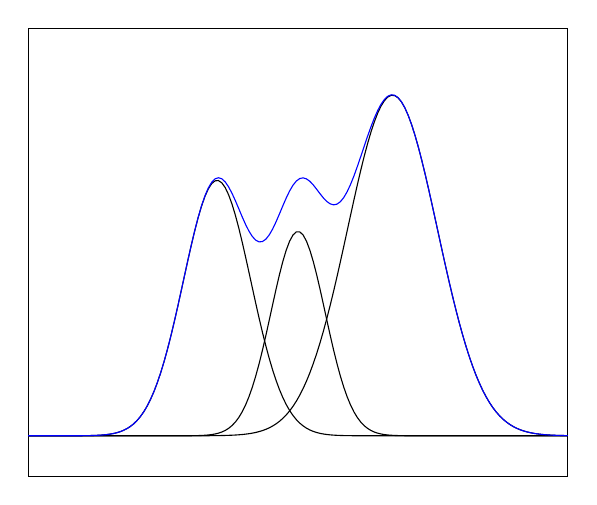
\begin{tikzpicture}
    \begin{axis}[
        ticks=none,
        xmin=-20, xmax=20,
        ymin=-1, ymax=10
    ]
        \addplot [domain=-25:25, samples=200, forget plot] {
            1/0.5*(2*pi)^0.5 * exp(-((x)^2)/2*0.25)
        };
        \addplot [domain=-25:25, samples=200, forget plot] {
            1/0.3*(2*pi)^0.5 * exp(-((x-7)^2)/2*0.09)
        };
        \addplot [domain=-25:25, samples=200, forget plot] {
            1/0.4*(2*pi)^0.5 * exp(-((x+6)^2)/2*0.16)
        };
        \addplot [blue,domain=-25:25, samples=200] {
            (1/0.5*(2*pi)^0.5 * exp(-((x)^2)/2*0.25))
            + (1/0.3*(2*pi)^0.5 * exp(-((x-7)^2)/2*0.09))
            + (1/0.4*(2*pi)^0.5 * exp(-((x+6)^2)/2*0.16))
        };
    \end{axis}
\end{tikzpicture}

\end{document}
